\let\negmedspace\undefined
\let\negthickspace\undefined
\documentclass[journal]{IEEEtran}
\usepackage[a5paper, margin=10mm, onecolumn]{geometry}
%\usepackage{lmodern} 
\usepackage{tfrupee} 

\setlength{\headheight}{1cm} 
\setlength{\headsep}{0mm}     

\usepackage{gvv-book}
\usepackage{gvv}
\usepackage{cite}
\usepackage{amsmath,amssymb,amsfonts,amsthm}
\usepackage{algorithmic}
\usepackage{graphicx}
\usepackage{textcomp}
\usepackage{xcolor}
\usepackage{txfonts}
\usepackage{listings}
\usepackage{enumitem}
\usepackage{mathtools}
\usepackage{gensymb}
\usepackage{comment}
\usepackage[breaklinks=true]{hyperref}
\usepackage{tkz-euclide} 
\usepackage{listings}                                        
\def\inputGnumericTable{}                                 
\usepackage[latin1]{inputenc}                                
\usepackage{color}                                            
\usepackage{array}                                            
\usepackage{longtable}                                       
\usepackage{calc}                                             
\usepackage{multirow}                                         
\usepackage{hhline}                                           
\usepackage{ifthen}                                           
\usepackage{lscape}

\begin{document}

\bibliographystyle{IEEEtran}
\vspace{3cm}

\title{11.2.9}
\author{AI25BTECH11003 - Bhavesh Gaikwad}
{\let\newpage\relax\maketitle}

\renewcommand{\thefigure}{\theenumi}
\renewcommand{\thetable}{\theenumi}
\setlength{\intextsep}{10pt} 

\numberwithin{equation}{enumi}
\numberwithin{figure}{enumi}
\renewcommand{\thetable}{\theenumi}


\textbf{Question}: AB is a line-segment. $\vec{P}$ and $\vec{Q}$ are points on opposite sides of AB such that each of them is equidistant from the points $\vec{A}$ and $\vec{B}$. Show that the line PQ is the
perpendicular bisector of AB.

\bigskip
 
\textbf{Solution:}\\
Since $\vec{P}$ has the same distance from $\vec{A}$ and $\vec{B}$,
\begin{equation}
    \norm{\vec{P}-\vec{A}} = \norm{\vec{P}-\vec{B}}
\end{equation}

We know
\begin{equation}
 \norm{\vec{W}}^2 = {\vec{W}^\top\vec{W}}   
\end{equation}

Squaring both sides in Equation 0.1,
\begin{equation}
(\vec{P}-\vec{A})^\top(\vec{P}-\vec{A}) = (\vec{P}-\vec{B})^\top(\vec{P}-\vec{B})
\end{equation}

After Simplifing, we get
\begin{equation}
    \vec{P}^\top(\vec{B}-\vec{A}) = \dfrac{1}{2}(\, \norm{\vec{B}}^2 - \norm{\vec{A}}^2 \,)
\end{equation}

Similarly for $\vec{Q}$,
\begin{equation}
     \vec{Q}^\top(\vec{B}-\vec{A}) = \dfrac{1}{2}(\, \norm{\vec{B}}^2 - \norm{\vec{A}}^2 \,)
\end{equation}

From A.5.1(Book),\\
The equation of perpendicular bisector of AB can be represented as
\begin{equation}
    \left( \vec{X} - \dfrac{\vec{A}+\vec{B}}{2} \right)^\top(\vec{B}-\vec{A}) = 0
\end{equation}


\begin{center}
    OR
\end{center}


\begin{equation}
    \vec{X}^\top(\vec{B}-\vec{A}) = \dfrac{1}{2}(\, \norm{\vec{B}}^2 - \norm{\vec{A}}^2 \,)
\end{equation}

\bigskip

A Point on line PQ can be represented as
\begin{equation}
    \vec{X} = \vec{P} + \lambda(\vec{P}-\vec{Q})
\end{equation}

Taking dot production with $\vec{B} - \vec{A}$ on both sides,
\begin{equation}
    (\, \vec{B} - \vec{A} \,)^\top \vec{X} = (\, \vec{B} - \vec{A} \,)^\top \vec{P} + \lambda(\, \vec{B} - \vec{A} \,)^\top(\, \vec{P} - \vec{Q} \,)
\end{equation}

\begin{center}
    OR
\end{center}

\begin{equation}
    \vec{X}^\top(\, \vec{B} - \vec{A} \,) = \vec{P}^\top(\, \vec{B} - \vec{A} \,) + \lambda(\, \vec{P} - \vec{Q} \,)^\top(\, \vec{B} - \vec{A} \,)
\end{equation}

\begin{equation}
   \vec{X}^\top(\, \vec{B} - \vec{A} \,) = (1+\lambda)\vec{P}^\top(\, \vec{B} - \vec{A} \,) - \lambda\vec{Q}^\top(\, \vec{B} - \vec{A} \,)
\end{equation}


From Equation 0.4 and 0.5,
\begin{equation}
    \vec{X}^\top(\, \vec{B} - \vec{A} \,) = (1+\lambda)\left[\dfrac{1}{2}(\, \norm{\vec{B}}^2 - \norm{\vec{A}}^2 \,)\right]  - \lambda\left[\dfrac{1}{2}(\, \norm{\vec{B}}^2 - \norm{\vec{A}}^2 \,)\right]
\end{equation}

\begin{equation}
    \vec{X}^\top(\vec{B}-\vec{A}) = \dfrac{1}{2}(\, \norm{\vec{B}}^2 - \norm{\vec{A}}^2 \,)
\end{equation}

\bigskip

Since, Equation 0.7 and 0.13 are same.
\begin{align*}
    \boxed{\text{Hence Proved , Line PQ is a perpendicular bisector to line segment AB.}}
\end{align*}

\bigskip
Example:\\
Assuming $\vec{A} = \myvec{1 \\ 0}$, $\vec{B} = \myvec{0 \\ 1}$, $\vec{P} = \myvec{0 \\ 0}$ and $\vec{Q} = \myvec{1 \\ 1}$

\begin{equation}
    \vec{B} - \vec{A} = \myvec{-1 \\ 1} \quad \& \quad \vec{P} - \vec{Q} = \myvec{-1 \\ -1} 
\end{equation}


\begin{equation}
    (\, \vec{B} - \vec{A} \,)^\top(\, \vec{P} - \vec{Q} \,) = 0
\end{equation}
Thus, Line PQ is perpendicular to line segment AB.\\\\

Let $\vec{M}$ be the midpoint of line segment AB.
\begin{equation}
    \vec{M} = \dfrac{\vec{A}+\vec{B}}{2} = \myvec{1/2 \\ 1/2}
\end{equation}

Equation of line PQ,
\begin{equation}
    \vec{X} = \vec{P} + \lambda(\, \vec{P}-\vec{Q} \,)
\end{equation}

\begin{equation}
    \vec{X} = \lambda\myvec{-1 \\ -1}
\end{equation}

$\vec{M}$ satifies equation 0.18, thus Line PQ passes through midpoint of line segment AB. Thus PQ bisects AB.

\begin{align*}
\therefore \text{Line PQ is a perpendicular bisector to line segment AB.}
\end{align*}


\begin{figure}[htbp]
    \centering
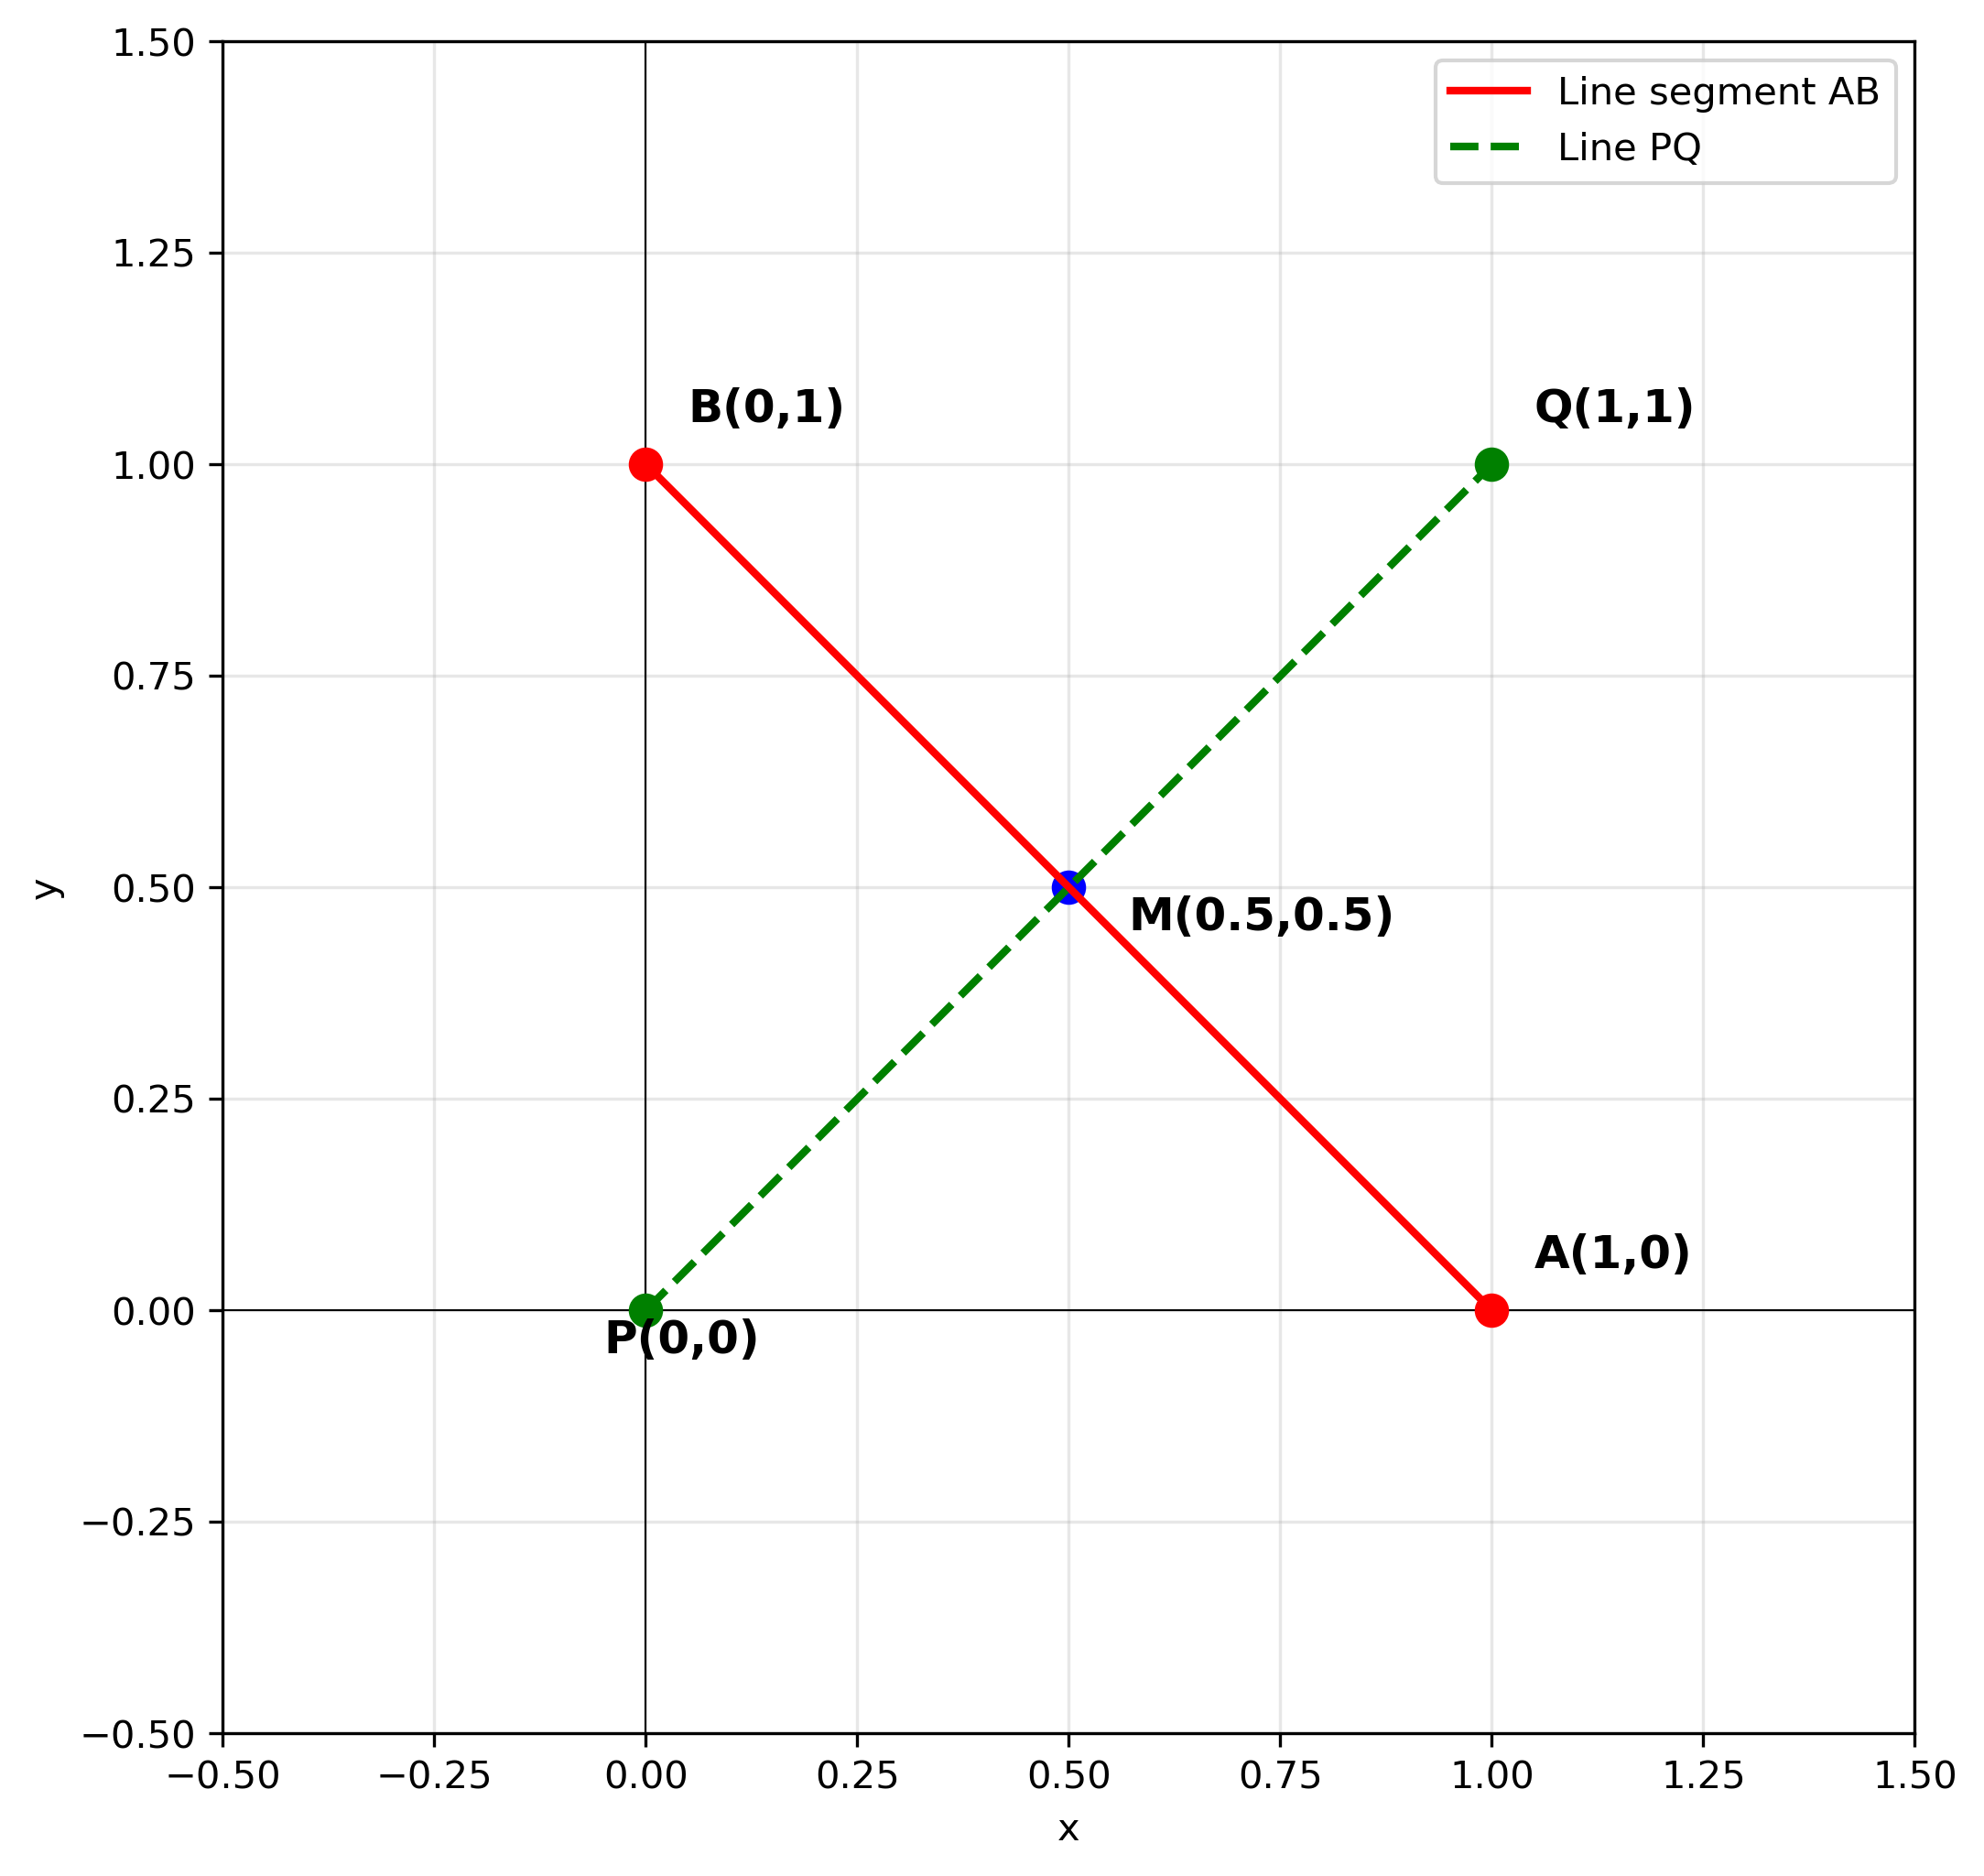
\includegraphics[width=\columnwidth]{figs/fig1.png}
    \caption{}
    \label{fig:figs/fig1.png}
\end{figure}

\end{document}  
